\logg{Torsdag 19. September}{09:00 til 16:00 (7 timer)}{
Møtte opp klokken 09:00 for å forbrede seg på et møte med \textit{RnD} gruppen som skulle ta sted klokken 10:00. I mellom disse to tidene gjorde studenten seg klar for å fylle ut kontrakt-avtale mellom studenten, universitetet og bedriften. \\

Dette ble fulgt opp av at møtet blir litt forsinket av en gruppemedlem er forsinket for møtet. Møtet startet da derfor 1030. På møtet ble studenten introdusert til den lineære matematikken bak abc-analyse formelen og hvordan denne matematikken blir brukt i bedriften. Her fikk studenten vite om diverse begreper som bedriften bruker; \textit{Activity}, \textit{Item}, \textit{Measure}, og \textit{Cost}. Aktivitet refererer til hvilket stadiet produktet er i. Om den er i transport, ligger i et varehus, eller rett og slett rotner. Produkt refererer til Hvordan produkt som man snakker om. Det kan være både gulrøtter og treverk, som eksempel. Måling er hva man måler absert på hva kost er. Kost kan variere om hva det er. Det kan være hvor mye CO2 utslipp produktet påfører, eller hvor mye penger dette produktet koster å transportere eller lagre. 

\begin{figure}[H]
\centering
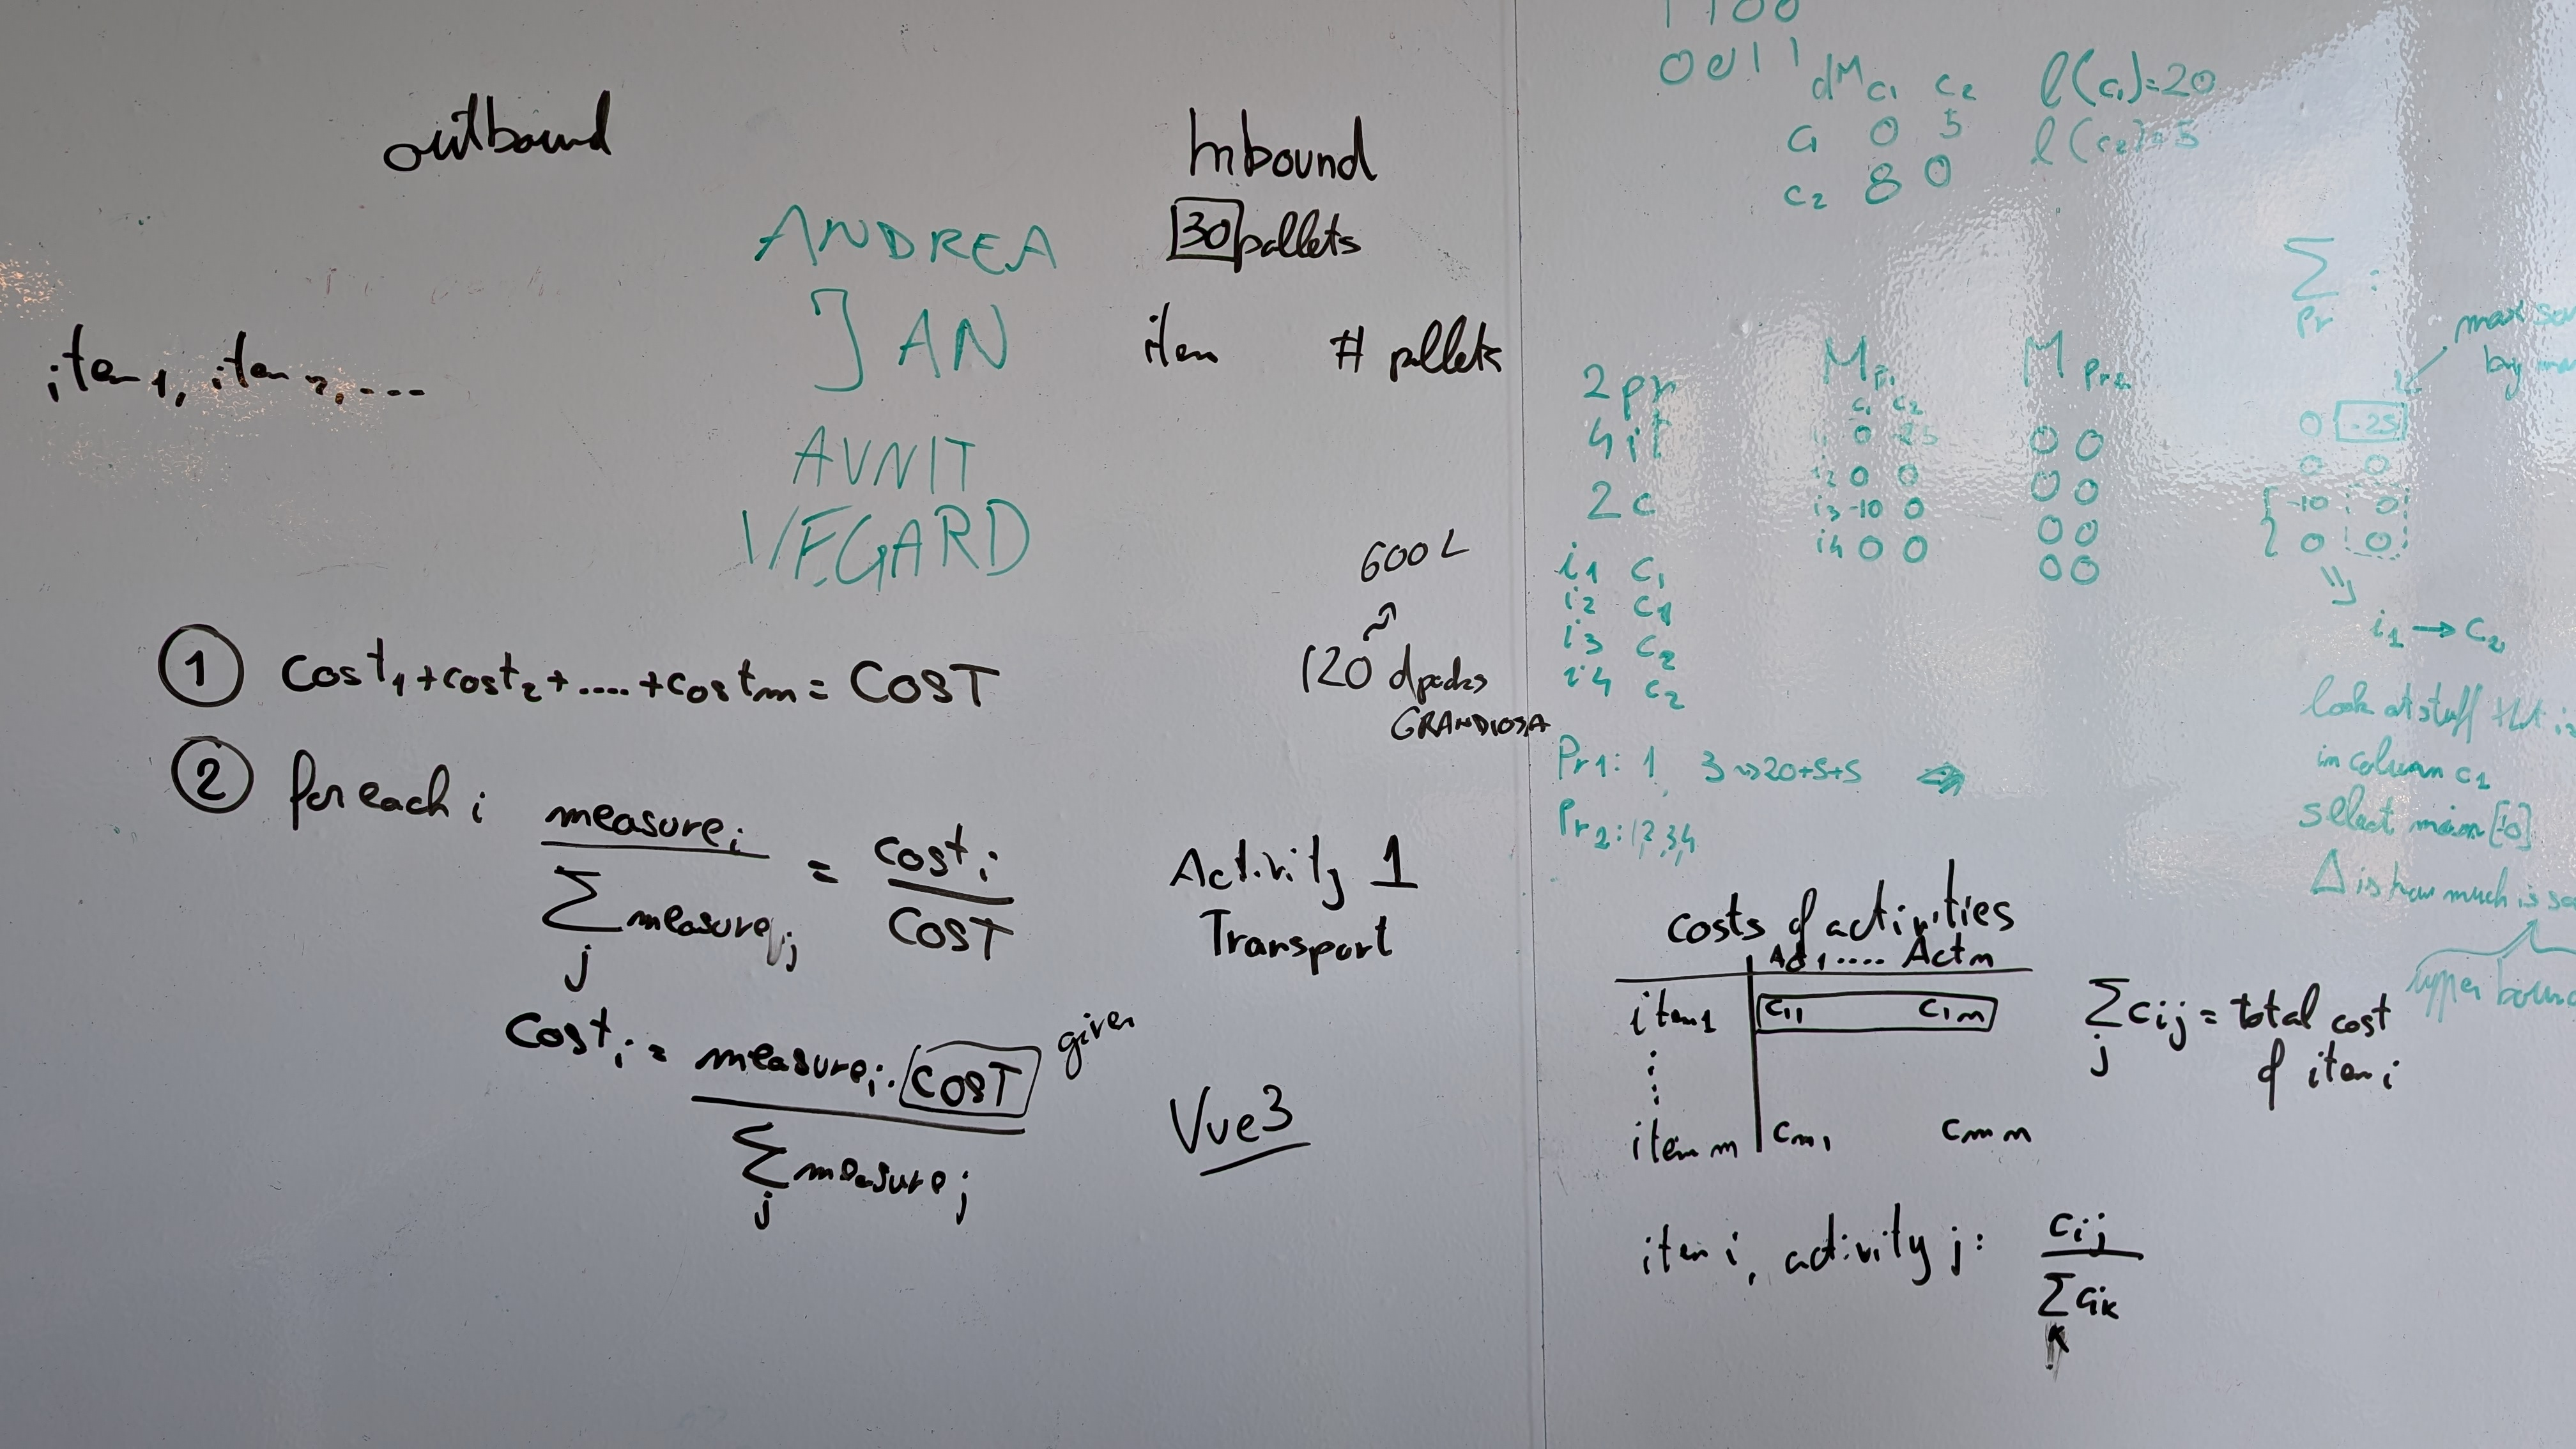
\includegraphics[width=0.50\linewidth]{ukentlige logger/images/uke 2/abc_analysis_basics.jpg}
\caption{\label{fig:downloads}Skisse over abc-analyse.}
\end{figure}

Etter møtet begynte studenten å fortsette jobben på databasen og trace-insight applikasjonen fra gårsdagen. Studenten fikk hjelp av en ansatt på bedriften. Det viser seg at trace-insight sin dokumentasjon var skrevet feil, og noe av koden ikke fungerte lenger. Dette gjorde det naturligvis vansklig for studenten å få startet opp applikasjonen. Den ansatte rettet da opp i feilen i koden og dokumentasjonen og \textit{pushet} det til repositoriet slik at studenten kunne \textit{pulle} det. 

Studenten fikk også hjelp til databasen, ettersom når dataen fra dump-filen ble gjennopprettet, ble ikke all dataen det. Noe som gjorde at studenten fikk hjelp til å opprette all dataten. Resultatet er ikke bekreftet ettersom det tar lang tid å opprette denne dataen (ingen vet hvorfor det tar så lang tid). \\

Etter at alle applikasjonene fungerer og databasen jobber med å gjenopprette dataen, begynte studenten og medstudentene å se på matematikken bak abc-analysen, for å kunne få en dypere forsåelse på hvordan den brukes. Dette ble gjort ved å se på diverse caser som kan skje. Her satt studentene og gjorde matte for å forså hvordan formelen fungerer.\\

Etter at studentene kom fram til en stopp, bestemte studenten Vegard Arnesen Mytting å dra hjem. Ettersom klokken var over 16:00. 
}\\\\\\